\documentclass{article} % review option
\usepackage[latin1]{inputenc}

\usepackage{graphicx}
\graphicspath{{./}{./images/}}
\usepackage[indention=10pt]{subfig}
 
\renewcommand{\topfraction}{1}
\renewcommand{\bottomfraction}{1}
\renewcommand{\textfraction}{0}
\renewcommand\floatpagefraction{0}

\usepackage{amssymb}
\usepackage{amsmath}
\usepackage{enumerate}

\usepackage{hyperref}
\usepackage[]{algorithm2e}

\newtheorem{theorem}{Theorem}
\newtheorem{definition}{Definition}
\newtheorem{proof}{Proof}



\begin{document}
\title{Data-driven measure of convergence for word embeddings}
\author{
  Martinez-Ortiz, Carlos
  \and
  Attema, Jisk
  \and
  Bos, Patrick
  \and
  Kenter, Tom
}

\maketitle

\begin{abstract}
Word embeddings have been used in a wide range of applications. It is generally agreed that training a word embedding requires a significant amount of data, however it is never entirely clear how much data is enough for the word embedding to capture the semantic structure of the language it is being trained with. Specific tests, based on word analogies, have been used to decide when a word embedding has captured enough of the language structure to be considered meaningful. However this approach has several issues, amongst others the language specificity of such tests.

In this paper we propose a completely data-driven method for determining the level of convergence of a semantic model, which enables us to train semantic models with enough data for the model to capture the semantic structure of language and stop the training when the model does not benefit significantly from the additional data. The proposed method measures the amount of change induced by each additional batch of data used to train the model; the internal structure of the model will continue to change as long as the model is still learning. Once the internal structure of the model stops changing, then the model can be considered as \textit{stable} and the training can stop.

The proposed method can be particularly useful when a limited amount of data is available or when the available data should be divided to train several models.

We compare our method with existing word analogy tests and show how our method still performs well in situations where word analogies are unable to perform as expected.
\end{abstract}

\section{Intoduction}
\label{sec:introduction}
Since their introduction \cite{Mikolov_CS2013}, word embeddings have become increasingly popular and have been used for a wide range of applications \cite{Mikolov_CoRR2013, Kim_CoRR2014, Levy_CNLL2014, Cordeiro_ACL2016, Smith_ICLR2017}. Word embeddings are often trained using large data sets, such as the Google News corpus\footnote{\url{https://code.google.com/archive/p/word2vec/}}, incorporating 100 billion words. The generally accepted approach when training word embeddings is the more data, the better, and there does not appear to be any consensus on the minimum amount of data required to train a word embedding model which yields good results. A widely accepted method for evaluating word embeddings is by testing their performance in analogy tests: \textit{man : woman :: king : \textbf{queen}}. Data sets for testing analogies are widely available\footnote{See \url{https://aclweb.org/aclwiki/State_of_the_art}}. However there are several known issues with such tests \cite{Speer_Blog2016}:

\begin{itemize}
 \item \textbf{Language specific} - analogies are usually language specific -- training a word embedding model on a language different from that of the analogies will obviously lead to failing the test;
 \item \textbf{Domain specific} - analogies usually fall in a particular knowledge category. For instance the following analogy: \textit{Athens : Greece :: Baghdad : Iraq}, is specific to Geographical facts; a semantic model trained on a data set which does not contain such knowledge (which never mentions these locations) is bound to fail this test. At the same time, a word embedding may have already learnt a domain specific analogy, such as \textit{electron : electricity :: photon : light}, but if this analogy is not reflected on the analogy test set, there is no way to know the semantic model already incorporates this knowledge;
 \item \textbf{Constrained by vocabulary} - because word embeddings typically have a set vocabulary; analogies which use out-of-vocabulary words, will always fail. Domain and language specific issues can be considered specific instances of constrained vocabulary issues.
\end{itemize}

Furthermore, recent criticisms question the suitability of semantic models to capture the relations in the language \cite{Hellrich_COLING2016}. However the quality measures proposed there are still language specific and thus suffer from the same limitations.

These issues can be addressed, for instance, by translating the analogy test sets, discarding analogies which are irrelevant for the data being used, constructing analogies suitable for a domain, etc. However all of these approaches are labour intensive and must be hand crafted for each training data set. This work is motivated by the desire to find a data-driven method to validate word embeddings. The data-driven method introduced here does not rely on the vocabulary and thus does not require translation or creation of new test sets in order to function. This makes our approach effectively language independent.

The data-driven method for word embedding evaluation measures the amount of change in the semantic space at every stage of the training. Large variation in the semantic space indicates that the model has acquired a large amount of knowledge from a given batch of data. Small variation in the semantic space indicates that the given batch of data has contributed little new information to the model. Once the variation in the model falls below a given threshold, the model is assumed to have assimilated enough information from the data to be able to capture the semantic structure of the data set.

This method may also be particularly useful in cases where the available data needs to be divided to allow for diachronic data analysis. In such cases there is a clear trade-off between the volume of data used to train the model and the temporal resolution of the analysis: data slices spanning longer periods of time contain more data and produce better models; on the other hand, data slices spanning shorter periods of time will allow a more detailed temporal resolution. The data-driven method allows us to find the right balance for such scenarios.

This paper is structured as follows: Section \ref{sec:method} describes the data-driven procedure for measuring convergence of word embeddings; Section \ref{sec:experiments} describes the setup used to evaluate word embedding convergence; Section \ref{sec:results} discusses the evaluation; concluding remarks are presented in Section \ref{sec:conclusion}.

\section{Method}
\label{sec:method}

We will start by giving a brief overview of how semantic models work, more details can be found in the original papers \cite{Mikolov_CS2013}. A semantic model ($M$) works by creating a semantic space in which each word ($w$) in the known vocabulary ($V$) is represented by a vector. This semantic space has $N$ dimensions. The number of dimensions is set at the beginning of the training process. The size of the vocabulary, is also determined from the start. Note that it is not unusual to restrict the vocabulary size to only include words which appear frequently (more than $k$ times) in the corpus.

To find the semantic space vector --- or \textit{embedding} --- of a word, we apply the following procedure:

Any given word $w$ in the vocabulary can be represented in \textit{vocabulary space} as a vector of size $V$ using \textit{one-hot} encoding. The linear transformation from vocabulary to semantic space is represented by an embedding matrix $S$ of size $NxV$. We can use matrix $S$ to find the embedding of $w$, which we call $e_w$:

$$e_w = S \cdot w$$

where vector $e_w$ is of size $N$. Words which have similar meaning will be located close by in this semantic space. As pointed in \cite{Hellrich_COLING2016}, such relations are questionable for low quality models, however we work with the assumption that larger volumes of data will provide sufficient quality models for these relations to be reasonably meaningful. Word similarity is usually measured using cosine similarity \cite{Kim_CoRR2014}. The semantic model learns the structure of the semantic space by analysing sentences in the corpus and updating the $S$ matrix.

We are interested in finding a matrix $S$ which is a good representation of our data. As we add more data to our semantic model, there will be different versions of $S$ changing over time: $S_1$, $S_2, ..., S_t$. By measuring the amount of change between any two consecutive models, $M_{i-1}$ and $M_i$, we can know how much the model needed to adapt to between $t=i-i$ and $t=i$ to fit the new data presented to the model. As some point in time $t=t^\ast$, the difference between the two models, $M_{t^\ast-1}$ and $M_t^\ast$, will be small enough that we can consider the two models to be equivalent.

We say that two models are equivalent when the local relations from one space are preserved in the other. This can be understood as that there exists a transformation to map between the two spaces.

In order to compare any two points along the training time, $A$ and $B$, we use the two versions of their embedding matrices, $S_A$ and $S_B$. We want to find a transformation matrix such that:

$$S_B \approx S_A \cdot T$$

The transformation matrix $T$ can be found using the procedure described in Pseudocode 1:

\begin{algorithm}[H]
  \ForEach{ dimension $i$ in the embedded space }{
    $\widehat{i_A}$ $\leftarrow$ unit vector along the i-th dimension of the embedded space $S_A$ \;
    $W_i$ $\leftarrow$ $\widehat{i_A}$ projected back into vocabulary space \footnote{To convert $\widehat{i_A}$ back into vocabulary space, we take the product of the embedded vector and the inverse of embedding matrix.} \footnote{If the vocabularies are different we need to convert $W_i$ to the other vocabulary} \;
    $T_i$ $\leftarrow$ $W_i$ projected in embedded space $S_B$ \;
    i-th dimension of $T$ $\leftarrow$ $T_i$ \;
  }
 \caption{Find $T$ to map from $S_A$ to $S_B$}
\end{algorithm}

$T$ will be of size $NxN$.

Alternatively, one can calculate $T$ using the following equation for each column $T_i$ of $T$:

$$T_i = S_B S_A^{-1} \widehat{i_A} $$

where $\widehat{i_A}$ is the unit vector along dimension $i$ in the semantic space defined by $S_A$.

Figure \ref{fig:transform} depicts how the transformation matrix is built.

\begin{figure}
 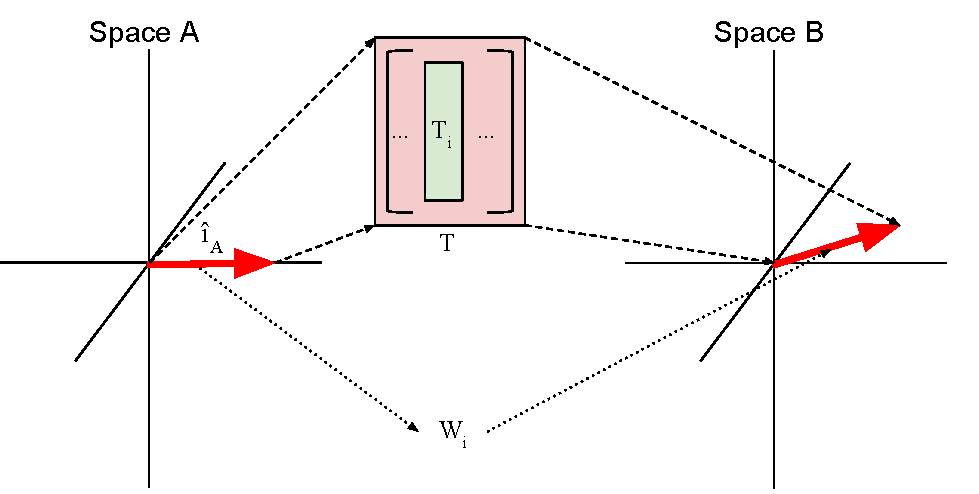
\includegraphics[width=\textwidth]{transformMatrix.pdf} 
 \caption{The $i$-th dimension transformation matrix $T$ ($T_i$), represents vector $\widehat{i_A}$ transformed from space defined by $S_A$ to from space defined by $S_B$.}
 \label{fig:transform}
\end{figure}

We will use the transformation $T$ to measure how much the embedded space has changed between times $A$ and $B$. To ensure that our measure is symmetric, we will calculate two transformation matrices, $T(A,B)$ to go from $A$ to $B$ and $T(B,A)$ to go from $B$ to $A$. We call the element-wise product of these two matrices the convergence matrix:

$$D(A,B) = T(A,B) * T(B,A)$$

It is important to mention that the convergence matrix will be equal the identity matrix if the space embeddings $S_A$ and $S_B$ are equivalent \footnote{have we defined what do we mean by equivalent?}. This follows from the fact that $T(X,Y)$ will be be the identity when $X$ and $Y$ are equivalent. Therefore, given $A$ and $B$ are equivalent, $T(A,B)$ and $T(B,A)$ will both be the identity, and thus $D(A,B) = T(A,B) * T(B,A)$ will also be the identity. \textbf{NOTE: think / check if the element-wise multiplication makes sense, as pointed out by Patrick.}

We use $D(A,B)$ measure the change in the semantic space in two different ways:

 - By taking the normalized trace of $D(A,B)$ - this will be equal to 1 if $S_A$ and $S_B$ are equivalent and yield a value between 0 and 1 if they are different. We call this \textit{convergence score}.
 - By looking at the values in the main diagonal of $D(A,B)$ - these values will be equal to 1 if $S_A$ and $S_B$ are equivalent and yield a value between 0 and 1 if they are different. This is similar to looking at the trace, but it provides additional information regarding the changes in the structure of the semantic space: are all vectors in the semantic space changing? Or are some of these vectors stable while others are changing significantly? We call this \textit{diagonal convergence scores}, and they provide not only information regarding whether the semantic space is changing, but also how it is changing.

\section{Experiments}
\label{sec:experiments}
In this section we describe the experimental process we have followed to validate our approach. For this experiment we used the Times news paper archives (\textbf{I need to ask Jose how can we reference the corpus}) between 1900 and 1980. We trained a semantic model, using gensim word2vec implementation, using CBOW. We set the dimensions on the semantic space to 300 ($N = 300$).

The vocabulary was limited to use a maximum of 1GB of memory; further, \textit{nltk} was used to remove non-words and stop-words \cite{Bird_NLP2009}. The resulting models had a maximum vocabulary size of 22,000 words. Notice that stop-word removal yielded a better final model with our data, but it does not affect the calculation of the convergence matrix.

We used batches of 10,000 sentences taken from randomly selected years in the corpus. After each batch is added to the model being trained, a snapshot of the embedding is taken. We continue to feed batches to the model until it has been trained with 10 million sentences.

We use $D(A,B)$ to compare snapshots. For comparison, we also use the Google "questions-words" analogy data set \cite{Mikolov_CS2013}\footnote{\url{https://aclweb.org/aclwiki/Google_analogy_test_set_(State_of_the_art)}}. It should be mentioned that some of the analogy tests failed for every one of our trained models because some words in those tests were not present in our corpus (more specifically, they were not present with enough frequency to be part of the vocabulary in our models). For example, even after training with 10 million sentences, our model fails for the analogy: \textit{London : England :: Montevideo : Uruguay}. This is however not surprising as \textit{Montevideo} appears only a 87 times in the first million sentences (for reference, London appears in 21,000 sentences). Notice that the proposed measure calculates the difference between two embeddings, while the question words evaluates the individual accuracy of a given model.

\section{Results}
\label{sec:results}

Figure \ref{fig:scores} shows the convergence score (blue) as the number of sentences increases, and the Google accuracy (green). After $10^6$ sentences have been used for training the model, there is a rapid increase in the convergence score. This indicates that the vectors defining the semantic space are becoming more stable. Training the model with additional sentences will produce little change in the model.

On the other hand, the Google accuracy score increases slowly but steadily. However, it requires a large number of sentences to increase the performance of the model. Depending on the application, there might be a trade off between the cost of using additional data and the benefit of doing so (notice that such a cost may not be economical but in terms of time, availability of data, or otherwise). In such cases it may be beneficial to stop once the cost/benefit balance crosses a certain point.

\begin{figure}
 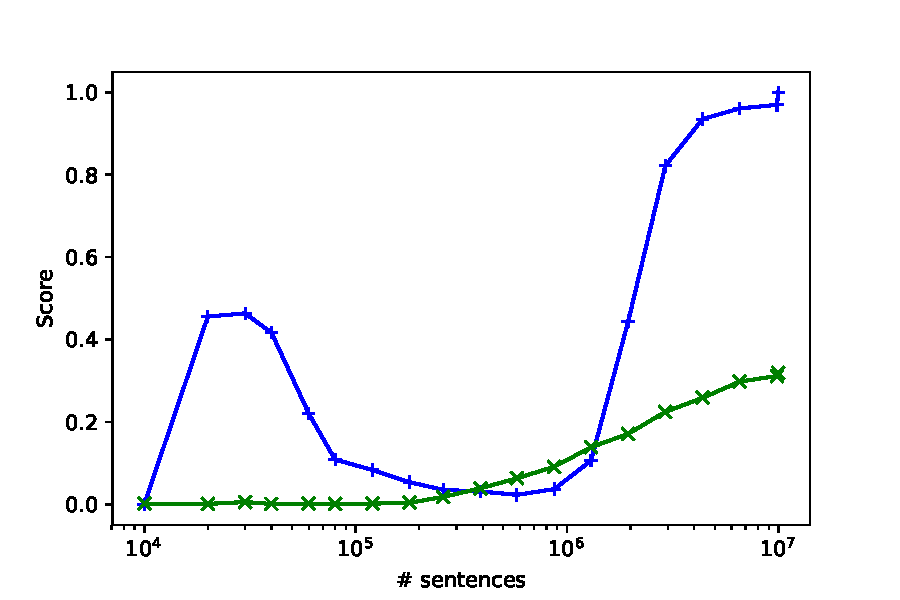
\includegraphics[width=\textwidth]{scoresVsNoSentences.pdf} 
 \caption{xxx}
 \label{fig:scores}
\end{figure}

At around $2 * 10^4$ sentences, there is a local maxima on the convergence score, but its value drops down at around $10^5$ sentences only to increase again at $10^6$ sentences. Such behaviour is indeed confusing; here we use the diagonal convergence scores gain some insight.

Figure \ref{fig:spreadDiagonal} shows the values on the diagonal of diagonal convergence scores as the number of sentences increases. Each line represents the convergence score for one particular dimension of the semantic space. What we see here is that around $2 * 10^4$ sentences there is wide variety of values for the convergence scores -- some dimensions of the semantic space are relatively stable (high convergence scores) while others are undergoing significant change (low convergence scores). As more sentences are added to the model, the changes in semantic model become more widespread, until finally the model becomes globally stable. \textbf{TODO -- Discuss: Why is Google Accuracy score so low ?}

\begin{figure}
 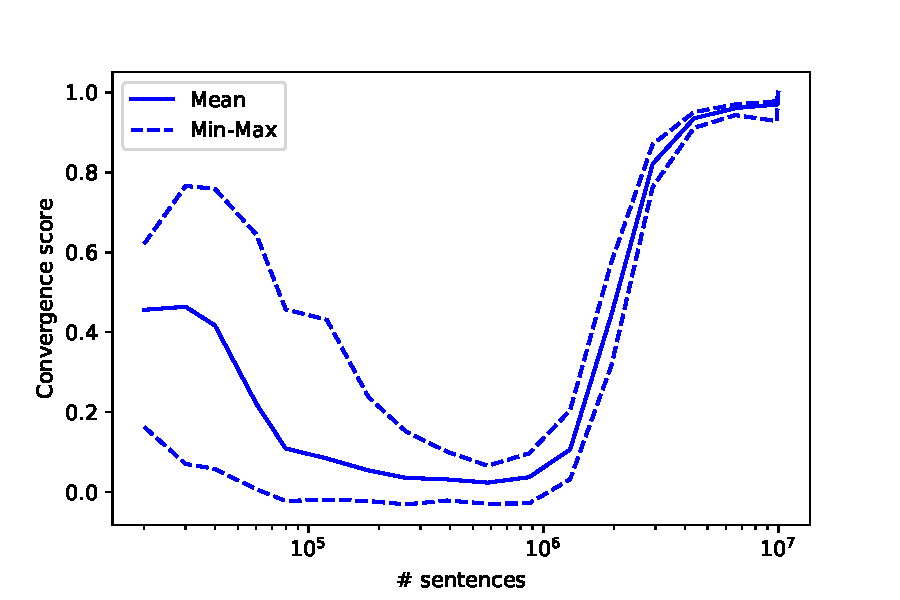
\includegraphics[width=\textwidth]{spreadDiagonalValues.pdf} 
 \caption{xxx}
 \label{fig:spreadDiagonal}
\end{figure}

\subsection{Temporal corpus slicing}
\label{subsec:temporal_corpus_slicing}
Semantic models have been used for diachronic analysis of vocabulary \cite{Martinez_Histo2016,Hellrich_COLING2016} \textbf{Add more refs from \cite{Hellrich_COLING2016}}. In such cases a corpus must be divided in temporal slices. Each of these slices will contain a subset of the corpus, with documents from a specific period (e.g. documents written between 1900 - 1905). This imposes a constraint in the volume of data available to train the model. In such scenario, the trade off between accuracy and data availability becomes evident: slices covering shorter time spans (e.g. a single year) will be more useful for temporal analysis of the data (e.g. allowing to identify the year when a change in the language took place); at the same time, the model will have less data available for training, thus compromising accuracy.

In order to find the optimal number of years to be used for temporal slices on the Times corpus described above, we trained semantic models, adding data in chronological order from 1900 onwards, and taking snapshots every 1/2 million sentences. The following figure shows the convergence score for these models. The Google accuracy score is also included for reference.

\begin{figure}
 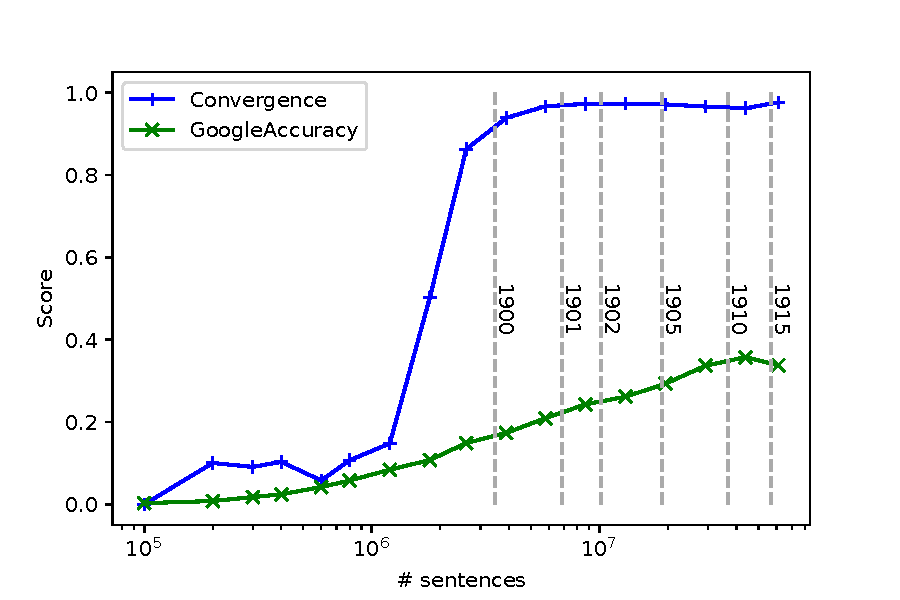
\includegraphics[width=\textwidth]{diachronicSlices.pdf} 
 \caption{xxx}
 \label{fig:diachronic}
\end{figure}

As it can be seen, after the model has been trained with 5 million sentences, there is a noticeable increase in the convergence measure, indicating that the model has stabilized. This is a period equivalent to two years; from this we conclude that using two year temporal slices is suitable for this dataset.

\section{Conclusion}
\label{sec:conclusion}
In this paper we have presented a data-driven method for measuring convergence of semantic models. This approach determines when a semantic model has been trained with enough data to capture the semantic structure of the data. This is useful when there is a trade off between longer training and more accurate models.

The convergence scores can be visualized as a single value over time, as shown on Figure \ref{fig:scores}, or as a collection of values as shown on Figure \ref{fig:spreadDiagonal}. The first form of visualization is more straight forward, while the second provides additional insight into the structure of the semantic space as a whole.

This approach is entirely data-driven and does not depend on previous knowledge of the language being modelled or on a manually translated reference corpus. This will help remove previously existing limitations in the application of semantic models.

%\section{Notes}
%\begin{itemize}
%\item Add a clarification (definition) of what it means for two spaces to be equivalent:
%  \begin{itemize}
%  \item Relations in one space are preserved in the other
%  \item It is basically just a rotation
%  \end{itemize}
%   
% \item "Known issues:" restructure (maybe into one thing)
%
% \item  Pseudocode 
% \begin{itemize}
%  \item Add picture (how would it look like)
%  \item Add intuitive / concrete example (using a word)
% \end{itemize}
%
% \item Separate repo for the code
%
% \item Move "We use D(A,B)..." to Method section (together with clarification of definition above)
% \item Add: we used CBOW (or skip gram)
% 
% \item Figure 2 
% \begin{itemize}
%  \item density plot
%  \item xaxis should be No. sentences
% \end{itemize}
%
% \item Figure 3
%  \begin{itemize}
%  \item add axis No. sentences
%  \item add discussion "why is google score low"
% \end{itemize}
%
% \item Add in introduction why we do this more strongly
%
% \item Venues:
% \begin{itemize}
%  \item LREC
%  \item IEEE
%  \item NIPS
%  \item PR ?
%  \item http://cs.rochester.edu/~omidb/nlpcalendar/
% \end{itemize}
%
%\end{itemize}

\bibliographystyle{plain}
\bibliography{shico}


\end{document}
